\chapter{Shapes}

Nu je weet hoe je een punt op het scherm kan tonen, zijn meer complexe figuren ook niet moeilijk. (Indien niet, kijk dan nog eens naar hoofdstuk \ref{chapter:positions}.) Je kan de meest voorkomende wiskundige vormen op het scherm tonen. De classes om dat te doen staan in de groene map Esenthel Engine $\Rightarrow$ Math $\Rightarrow$ Shapes.

Niet alle figuren kan je in een 2D programma gebruiken. Sommige classes, zoals \eeClass{Ball} en \eeClass{Tube}, zijn bedoeld voor 3D toepassingen. In 2D kan je \eeClass{Circle}, \eeClass{Edge} (lijn), \eeClass{Quad}, \eeClass{Rectangle} en \eeClass{Triangle} gebruiken.

\section{Circle}
Om een cirkel te tekenen heb je een straal(r) en een positie(pos) nodig. Die straal is een \eeClass{float}, de positie is een \eeClass{Vec2}. Je kan die op meer dan 1 manier instellen:

\begin{code}
// via de constructor, met r(float), pos.x(float), pos.y(float)
Circle c(0.1, 0, 0);

// via de constructor, met r(float), pos(Vec2)
Circle c(0.1, Vec2(0, 0));

// tijdens de duur van het programma
c.set(0.1, 0, 0);
c.set(0.1, Vec2(0, 0));

// zonder de set functie
c.r = 0.1;
c.pos = Vec2(0, 0);
\end{code}

\subsection{Functies}
Je kan ook het oppervlak of de omtrek van de cirkel opvragen via functies, of de cirkel op het scherm tonen:

\begin{code}
// oppervlak en omtrek
float opp = c.area();
float omtrek = c.perimeter();

// een blauwe cirkel op het scherm tonen
c.draw(BLUE);

// enkel een blauwe omtrek tonen
c.draw(BLUE, false);
\end{code}

Er is iets opmerkelijks aan de hand met de \eeFunc{draw} functie! Je kan ze zowel met \'e\'en als met twee argumenten gebruiken. Om te weten hoe dat komt, moet je naar de definitie van die functie kijken (je vindt die in Esenthel Engine $\Rightarrow$ Math $\Rightarrow$ Shapes $\Rightarrow$ Circle):

\begin{code}
void draw(C Color & color, Bool fill = true, Int resolution = -1) C;
\end{code}

Je ziet dat het eerste argument een \eeClass{Color} moet zijn. Het tweede argument is een \eeClass{bool} met de naam `fill'. Je zou dus al kunnen vermoeden dat die dient om de cirkel gevuld te tekenen. Dit argument heeft ook een standaard waarde: true. Daarom is het niet nodig om de draw functie met beide argumenten te gebruiken als je akkoord gaat met de standaard waarde. Enkel wanneer je een cirkel niet gevuld wil tekenen, geef je false door aan de functie.


\begin{note}
Ook het derde argument: `resolution' is optioneel. Experimenteer met verschillende waarden om te ontdekken wat je hier mee kan doen.
\end{note}

\subsection{Rekenen}
Je kan de operators \eeOpp{+=}, \eeOpp{-=}, \eeOpp{/=} en \eeOpp{*=} gebruiken om te `rekenen' met cirkels. Hierbij heb je twee mogelijkheden: een \eeClass{float} past de straal aan, een \eeClass{Vec2} de positie.

\begin{code}
Vec2 pos(0.1, 0);
Circle c(0.1, pos);

// verplaats de cirkel 0.1 naar rechts
c += pos;
// verplaats de cirkel 0.2 naar beneden
c -= Vec2(0, 0.2);
// verdubbel de straal van de cirkel
c *= 2;
\end{code}

\subsection{Oefeningen}
Maak de volgende afbeelding na door cirkels op je scherm te plaatsen. Als uitbreiding kan je ook eens naar de functie `\eeFunc{drawPie}' kijken en een meer geschikte mond voorzien.

\begin{figure}[h]
\centering
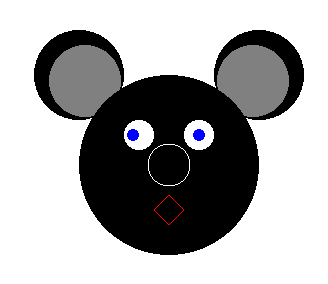
\includegraphics[width=0.4\linewidth]{../images/circle_exercise}
\caption[]{Let op de oogjes!}
\label{fig:pos2D}
\end{figure}

\section{Edge2}
Een \eeClass{Edge2} is een lijnstuk. De `2' is net zoals bij \eeClass{Vec2} belangrijk. Wanneer je die vergeet is je code wel geldig, maar dient die om een lijnstuk in 3D te tekenen. Om een \eeClass{Edge2} te defini\"eren heb je twee punten nodig, het begin en het eind. Esenthel bied je twee mogelijkheden om die in geven:

\begin{code}
Edge2 lijn1;
Edge2 lijn2;

// via vectoren
lijn1.set(Vec2(0, 0), Vec2(0.1, 0.1));

// dit kan ook met bestaande vectoren
Vec2 pos1(0.3, 0.6);
Vec2 pos2(0.1, 0.2);
lijn1.set(pos1, pos2);

// je kan ook alle x en y waarden afzonderlijk ingeven
lijn2.set(-0.4, 0.2, -0.7, 0.9;
\end{code}

Zoals je ziet heb je voor elk punt een x- en een y-co\"ordinaat nodig. Je kan die, zoals in het eerste voorbeeld, ingeven via een \eeClass{Vec2}. Of je kiest voor de tweede optie en geeft x1, y1, x2 en y2 in.

\subsection{Functies}
Ook een \eeClass{Edge2} heeft een aantal handige functies. Je kan al verwachten dat er een functie \eeFunc{draw()} bestaat:

\begin{code}
line1.draw(PURPLE    );
line2.draw(GREEN, 0.1); // stel ook de breedte in
line3.draw(GREEN, RED); // ga over van groen naar rood
\end{code}

Daarnaast kan je ook informatie over de lijn opvragen via bijvoorbeeld \eeFunc{center()}, \eeFunc{delta()}, \eeFunc{dir()} en \eeFunc{length()}. Je kan alle functies vinden in Esenthel Engine $\Rightarrow$ Math $\Rightarrow$ Shapes $\Rightarrow$ Edge.

\subsection{Oefeningen}

Via de functies \eeFunc{Sin()} en \eeFunc{Cos()} kan je de sinus en cosinus van een getal opvragen. Dit is vooral handig omdat dat getal bijvoorbeeld de tijd kan zijn. Via de tijd krijg je een geleidelijke verandering in de sinus en cosinus waarde. Beiden bewegen constant tussen -1 en 1. 

\begin{code}
float x = Sin(Time.curTime());
float y = Cos(Time.curTime());
\end{code}

\begin{enumerate}
\item De bovenstaande code helpt je met berekening van sinus en cosinus van de tijd. Maak nu een programma waarin je een lijn toont van in het midden van je scherm tot de huidige waarde van sinus en cosinus.
\item Pas de dikte van de lijn aan.
\item Zorg er voor dat de lijn dubbel zo snel beweegt.
\item Zorg er voor dat de lijn maar half zo lang is.
\end{enumerate}

Kijk eens in Esenthel Engine $\Rightarrow$ Math $\Rightarrow$ Shapes $\Rightarrow$ Edge. Je kan daar de functie \eeFunc{lerp(float s)} vinden. Deze functie heeft een getal tussen 0 en 1 nodig en geeft een punt in de lijn terug.

\begin{enumerate}
\item Definie\"er globaal een \eeClass{Edge2} en een \eeClass{float}, gelijk aan 0;
\item In de init functie laat je de lijn van -1, 0 tot 1, 0 lopen.
\item In de update functie verhoog je de float met \eeClass{Time.d()}. Wanneer de float groter is dan 1, dan stel je hem gelijk aan 0.
\item In de draw functie teken je de lijn in het zwart, met breedte 0.05. Je maakt een \eeClass{Vec2} die je de waarde geeft van de \eeFunc{lerp()} functie van je lijn, met als argument je float. Dit punt teken je rood, met eveneens een breedte 0.05.
\end{enumerate}

\textbf{(Uitbreiding)} Teken ook eens een driehoek op het scherm.

\section{Rect}
De laatste vorm die we bespreken is de rechthoek: \eeClass{Rect}. Waarschijnlijk is dit de vorm die je in je eigen programma's het meest zal gebruiken. Een rechthoek ligt immers ook aan de basis van veel andere elementen, zoals een button, een window en een afbeelding.

Na de laatste oefening weet je dat je, om een driehoek te tekenen, 3 posities nodig hebt. Logischerwijs zou je kunnen besluiten dat je voor een rechthoek 4 punten moet ingeven. Maar een rechthoek heeft een bijzondere eigenschap: het is een RECHThoek. Bijgevolg is het genoeg om de linkeronderhoek en de rechterbovenhoek in te geven. De rest kan daaruit afgeleid worden.

\begin{figure}[h]
\centering
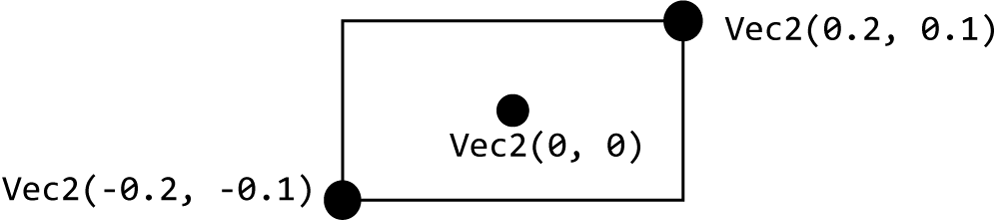
\includegraphics[width=0.8\linewidth]{../images/rectangle}
\caption[]{De hoeken van een rechthoek}
\label{fig:rect}
\end{figure}

De code voor deze rechthoek ziet er zo uit:

\begin{code}
Rect(Vec2(-0.2, -0.1), Vec2(0.2, 0.1)).draw(BLACK, false);
\end{code}

Zoals je ziet is er ook nu een draw functie, waarin het eerste argument de kleur is, en je daarna optioneel kan aangeven dat je de rechthoek niet wil vullen. Net zoals bij een edge heb je ook nu weer de mogelijkheid om de x- en y-co\"ordinaat afzonderlijk in te geven:

\begin{code}
Rect(-0.2, -0.1, 0.2, 0.1).draw(BLACK);
\end{code}

\subsection{Een bewegende Rect}
Omdat een rechthoek dikwijls aan de basis ligt van figuren die je op het scherm wil tonen, en die figuren in een spel nogal vaak bewegen, is het dikwijls handig om een eigen class te maken die intern een rechthoek gebruikt. In deze sectie maken een rechthoek die je kan bewegen via de pijltjestoetsen.

Rechthoeken hebben \'e\'en nadeel wanneer je ze vlot wil bewegen: we hebben de positie van de hoeken nodig in plaats van het midden van de rechthoek. Dat betekent dat we telkens twee punten moeten aanpassen voor elke verplaatsing. Daarom is het dikwijls eenvoudiger om een \eeClass{Vec2} te gebruiken om de positie te onthouden. We declareren ook een kleur, zodat een rechthoek zijn eigen kleur kan onthouden.

\begin{code}
class movableRect {
  Vec2 pos;
	Color color;
}
\end{code}

Deze class kunnen we uitbreiden met een create functie, een update functie en een draw functie. Via de create functie geef je de kleur en de startpositie door. De startpositie heeft een standaard waarde, dus wanneer je later de create functie gebruikt zonder een positie, dan staat de rechthoek in het midden van het scherm.

\begin{code}
void create(C Color & color, C Vec2 & pos = 0) {
  T.color = color;
	T.pos = pos;
}
\end{code}

\begin{note}
In deze functie staan nog enkele nieuwigheden. De ampersand geeft aan dat we color en pos als referentie doorgeven. De \eeFunc{C} betekent dat we de waarde niet zullen aanpassen. Je leert hierover meer in een van de volgende hoofdstukken. De letter \eeFunc{T} lost een praktisch probleem op. Zowel het functie-argument als de Color in de class zelf hebben als naam `color'. De compiler kan daarom niet weten wanneer je welke variabele bedoelt. Je zou ze beiden een verschillende naam kunnen geven, maar dat maakt de code moeilijker leesbaar. De elegante oplossing bestaat er in \eeFunc{T.} voor de variabele van de class toe te voegen. De T staat voor `this' en daarmee bedoelen we `deze class'. De versie zonder \eeFunc{T.} is bijgevolg de variabele die we als functieargument doorgeven.
\end{note}

In de update functie kunnen we de positie wijzigen via de pijltjestoetsen. Deze code heb je reeds gezien in hoofdstuk \ref{chapter:keyboardInteractie}.

\begin{code}
void update() {
	if(Kb.b(KB_LEFT )) pos.x -= Time.d();
	if(Kb.b(KB_RIGHT)) pos.x += Time.d();
	if(Kb.b(KB_UP   )) pos.y += Time.d();
	if(Kb.b(KB_DOWN )) pos.y -= Time.d();
}
\end{code}


Tot slot is er een draw functie nodig. Het is pas op deze plaats dat we, tijdelijk, een rechthoek maken. In dit geval is dat het meest praktisch, maar dat hoeft niet altijd zo te zijn. Het zou bijvoorbeeld kunnen dat je in de update functie wil controleren of de rechthoek iets raakt. In zo'n geval zou je waarschijnlijk ook een \eeClass{Rect} aan je class toevoegen.

\begin{code}
void draw() {
  Rect(pos - Vec2(0.2, 0.1), pos + Vec2(0.2, 0.1)).draw(color);
}
\end{code}

Zoals je ziet gebruiken we de positie `pos' bij het maken van de rechthoek. Die is namelijk het middelpunt. Aangezien we de hoeken linksonder en rechtsboven nodig hebben bij het maken van een rechthoek, kunnen we eenvoudig een waarde respectievelijk aftrekken en optellen. We zouden deze class nog wat meer flexibel kunnen maken door een `size' te onthouden.

Omdat dit de eerste maal is dat we een volledige class uitwerken in esenthel krijg je ze hieronder nog eens helemaal te zien. Let ook op de keywords public en private. Die zijn later belangrijk als je je code overzichtelijk wil houden.

\begin{code}
class movableRect {
private:
  Vec2 pos, size;
	Color color;
	
public:
  void create(C Color & color, C Vec2 & pos = 0, C Vec2 & size = Vec2(0.1, 0.1)) {
	  T.color = color;
		T.pos   = pos  ;
		T.size  = size ;
	}
	
	void update() {
		if(Kb.b(KB_LEFT )) pos.x -= Time.d();
		if(Kb.b(KB_RIGHT)) pos.x += Time.d();
		if(Kb.b(KB_UP   )) pos.y += Time.d();
		if(Kb.b(KB_DOWN )) pos.y -= Time.d();
	}
	
	void draw() {
		Rect(pos - size, pos + size).draw(color);
	}
}
\end{code}
	
\subsection{Oefeningen}

\begin{enumerate}
\item Maak in een programma de volgende afbeelding na:

\begin{figure}[h]
\centering
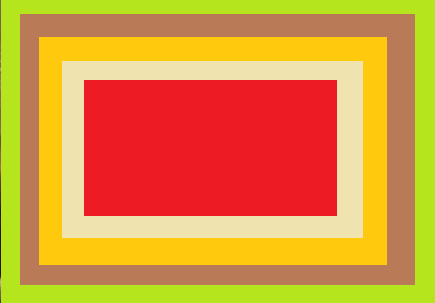
\includegraphics[width=0.4\linewidth]{../images/nested_rectangles}
\caption[]{Rechthoeken}
\label{fig:nested_rect}
\end{figure}

\item Voeg een roze vierkant toe van de class \eeClass{movableRect} die we hierboven voorstelden.
\item \textbf{(Uitbreiding)} Zorg dat het vierkant niet buiten het scherm kan bewegen.
\end{enumerate}

\section{Cuts}

Een functie die je vaak gebruikt in verband met shapes is \eeFunc{Cuts}. Er bestaan heel veel varianten op deze functie, maar de betekenis is steeds dezelfde: raken twee objecten mekaar of niet? Zo kan je controleren of een punt en een cirkel mekaar raken, of een cirkel en een rechthoek, twee rechthoeken, een driehoek en een lijn, enzovoort.

Om te controleren o een punt een cirkel raakt, gebruik je bijvoorbeeld de volgende code:

\begin{code}
Vec2 pos(0.1, 0.1);
Circle area(0.3, Vec2(0));

if(Cuts(pos, area)) area.draw(RED);
\end{code}

Natuurlijk is het in dit voorbeeld al duidelijk dat het punt de cirkel steeds zal raken. Maar ook de positie van je muiswijzer is een punt. Je zou dus het volgende kunnen schrijven:

\begin{code}
Circle area(0.1, Vec2(0));

if(Cuts(Ms.pos(), area)) area.draw(RED);
else area.draw(BLACK);
\end{code}

De code hierboven ligt aan de basis van vele interactiemogelijkheden. Dikwijls gebeurt dit in combinatie met andere controles. Probeer zelf eens te bedenken wat de volgende code doet:

\begin{code}
Rect button(Vec2(-0.2, -0.1), Vec2(0.2, 0.1));
bool hover = false;

// in een update functie:
if (Cuts(Ms.pos(), button)) {
  hover = true;
	if(Ms.bp(0)) exit();
} else hover = false;

// in een draw functie
if(hover) {
  button.draw(Color(0, 255, 0));
} else {
  button.draw(Color(0, 155, 0));
}
\end{code}

\subsection{Oefeningen}
\begin{enumerate}
\item Maak een programma met 3 cirkels (onder mekaar) waarvan je enkel de rand toont, tenzij de muiscursor zich in een van de cirkels bevindt. In dat geval teken je die cirkel gevuld.
\item Pas het vorige programma aan. Zorg er voor dat een cirkels langzaam naar rechts beweegt wanneer die zich onder de muiscursor bevindt.
\item Maak een integer `score'. Wanneer een cirkel de rechterkant van het scherm raakt, verhoog je de score met \'e\'en en plaats je de cirkel terug links.
\end{enumerate}

\textbf{(Uitbreiding) }Maak een eigen class die zich als een button gedraagt. Je kan vertrekken van het voorbeeld hierboven en een hover effect implementeren. (Extra uitdaging: de kleur kan ook geleidelijk veranderen.) Een button zal ook een tekst moeten tonen, dus je voorziet een create functie die de positie en die tekst instelt. Een meer algemene functie om te bepalen wat de button doet wanneer je er op klikt is nog niet voor nu, maar je kan natuurlijk altijd proberen.





